\documentclass[10pt,a4paper]{book}
\usepackage[utf8]{inputenc}
\usepackage{amsmath}
\usepackage{amsfonts}
\usepackage{amssymb}
\usepackage{minted}
\definecolor{mygray}{gray}{0.9}
\usepackage{graphicx}
\usepackage{hyperref}
\usepackage{enumitem}
\author{Nicolò Fornari}
\title{Security testing}
\newtheorem{remark}{Remark}
\begin{document}
\begin{document}
%\maketitle
\chapter{Memory}
Memory is just bytes of temporary storage space that are numbered with addresses. This memory can be accessed by its addresses, and the byte at any particular address can be read from or written to.\\\\
\emph{Pointers} are a special type of variable used to store addresses of memory locations to reference other information.
Because memory cannot actually be moved, the information in it must be copied. However, it can be computationally
expensive to copy large chunks of memory around to be used by different functions or in different places.A new block of memory must be allocated for the copy destination before the source can be copied. Pointers are a solution to this problem. Instead of copying the large block of memory around, a pointer variable is assigned the address of that large memory block. Then this small 4-byte pointer
can then be passed around to the various functions that need to access the large memory block.\\\\
The processor has its own special memory, which is relatively small. These portions of memory are called registers,and there are some special registers,one of the most notable is the EIP (extended instruction pointer).\\
The EIP is a pointer that holds the address of the currently executing
instruction. Other 32-bit registers that are used as pointers are the extended base pointer (EBP) and the extended stack pointer (ESP).
\section{Memory declaration}
When programming in a high-level language, like C, variables are declared using a data type. These data types can range from integers to characters to custom user-defined structures. One reason this is necessary is to properly allocate space for each variable.\\\\
In addition, variables can be declared in \emph{arrays}. An array is just a list of N elements of a specific data type. So a
10-character array is simply 10 adjacent characters located in memory. An array is also referred to as a \emph{buffer}, and a character array is also referred to as a \emph{string}.\\\\
One important detail of memory on x86 processors is the byte order of 4-byte words. The ordering is known as \emph{little endian}, meaning that the least significant byte is first.\\\\
For any string a zero, or null byte, delimiter is used to terminate it and tell any function that is dealing with the string to stop operations there.
\section{Program memory segmentation}
Program memory is divided into five segments: text, data, bss, heap, and stack. Each segment represents a special portion of memory that is set aside for a certain purpose.As a program executes, the EIP is set to the first instruction in the text segment. The processor then follows an execution loop that does the following:
\begin{enumerate}
\item Read the instruction that EIP is pointing to.
\item Add the byte-length of the instruction to EIP.
\item Execute the instruction that was read in step 1.
\item Go to step 1
\end{enumerate}
Write permission is disabled in the text segment, as it is not used to store variables, only code. This prevents people
from actually modifying the program code, and any attempt to write to this segment of memory will cause the program to alert the user that something bad happened and kill the program. Another advantage of this segment being read-only is that it can be shared between different copies of the program, allowing multiple executions of the program at the same time without any problems. It should also be noted that this memory segment has a fixed size, because nothing ever changes in it.\\\\
The \emph{data} and \emph{bss} segments are used to store global and static program variables. The data segment is filled with the initialized global variables, strings, and other constants that are used through the program. The bss segment is filled with the uninitialized counterparts. Although these segments are writable, they also have a fixed size.\\\\
The \emph{heap} segment is used for the rest of the program variables. One notable point about the heap segment is that itisn't of fixed size, meaning it can grow larger or smaller as needed.\\\\
The \emph{stack} segment also has variable size and is used as a temporary scratchpad to store context during function calls.
When a program calls a function, that function will have its own set of passed variables, and the function's code will be at a different memory location in the text (or code) segment. Because the context and the EIP must change when a
function is called, the stack is used to remember all of the passed variables and where the EIP should return to after the function is finished.\\\\
As the name implies, the stack segment of memory is, in fact, a stack data structure. When an item is placed into a stack, it's known as \emph{pushing}, and when an item is removed from a stack, it's called \emph{popping}. The ESP register is used to keep track of the address of the end of the stack, which is constantly changing as items are pushed into and popped from it.
Because this is very dynamic behavior, it makes sense that the stack is also not of a fixed size. Opposite to the growth
of the heap, as the stack changes in size, it grows upward toward lower memory addresses.
\begin{remark}
The EBP register is sometimes called the \emph{frame pointer} FP or \emph{local base pointer} LB.
The EBP is used to reference variables in the current stack frame.
\end{remark}
Each stack frame contains the parameters to the function, its local variables, and two pointers that are necessary to put things back the way they were: the \emph{saved frame pointer} SFP and the \emph{return address}.
The stack frame pointer is used to restore EBP to its previous value, and the return address is used to restore EIP to the next instruction found after the function call.
\chapter{Assembly}
\section{Registers}
\textbf{What are registers for?}
\begin{itemize}[noitemsep,nolistsep]
\item Store instructions
\item Store result of operations
\item Manipulate data in them (shift registers)
\end{itemize}
\textbf{Registers overview}\\\\
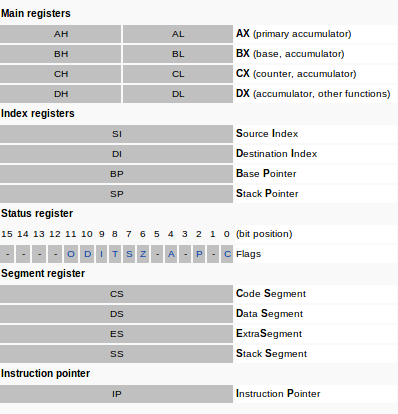
\includegraphics[scale=0.6]{registers.png}
\newpage
\textbf{Main registers}\\\\
\begin{tabular}{|c|c|c|c|}
\hline 
32 bit & 16 bit & 8 bit (high) & 8 bit (low) \\ 
\hline 
EAX & AX & AH & AL \\ 
\hline 
EBX & BX & BH & BL \\ 
\hline 
ECX & CX & CH & CL \\ 
\hline 
EDX & DX & DH & DL \\ 
\hline 
\end{tabular} 
\\\\
EAX, AX, AH and AL are called the \textbf{Accumulator} registers and can be used for I/O port access, arithmetic, interrupt calls etc.\\\\
EBX, BX, BH, and BL are the \textbf{Base} registers and are used as base pointers for memory access. This register is also sometimes used to store return value from an interrupt in. \\\\
ECX, CX, CH, and CL are also known as the \textbf{Counter} registers. \\\\
EDX, DX, DH, and DL are called the \textbf{Data} registers and can be used for I/O port access , arithmetic and some intrerrupt calls.

\newpage
\section{Hello world}
\begin{minted}[
bgcolor=mygray,
]{as}
section .data
	hello:     db 'Hello world!',10    ; 
	helloLen:  equ \$-hello             ; length 
	                                   ; to be explained

section .text
	global _start

_start:
	mov eax,4            ; (sys_write)
	mov ebx,1            ; standard output
	mov ecx,hello        ; offset into in ecx
	mov edx,helloLen     ; helloLen is a constant
	                     ;  
	int 80h              ; Call the kernel

	mov eax,1            ; (sys_exit)
	mov ebx,0            ; return code of 0 (no error)
	int 80h
\end{minted}
\\\\
Then in the terminal:\\\\
\begin{minted}[
bgcolor=mygray,
]{as}
nasm -f elf hello.asm
ld -m elf_i386 -s -o hello hello.o
\end{minted}
\\\\
Note that the elf\_i386 is necessary as we are writing 32 bit assembly code in a 64 bit architecture.
\newpage
\section{Introducing concepts with an example}
Let's look at some short code and describe what it does. Please note that it's pseudocode, it's not made for a specific architecture or language and various symbols can differ, the principle however, remains the same\\\\
\begin{minted}[
bgcolor=mygray,
]{as}
MOV A, 2000
LOOP:
ADD A, #5
JNL A, #200, LOOP
MOV 2001, A
\end{minted}
\\\\
The first instruction will move the number from the memory cell with address 2000 to a register A - it's a temporary location, where the processor stores numbers. It can have many registers like this. The second line contains something called a \textbf{label}: it's not an instruction, it's simply a mark in the source code that we may use later.\\\\
On the third line, there's an ADD instruction, which adds two numbers together. The operands are register A and number 5 (the \# mark before tells the assembler that it's number five, not a number in the memory cell with address 5). And remember? We stored the value from memory location 2000 in the A register, so whatever the value is, this instruction will add the number 5 to it.\\\\
The following instruction is called a \textbf{conditional jump}: the processor will test some condition and based on the result, it will jump or not. In this case, the condition is whether a given number is not larger than another one (JNL = Jump (if) Not Larger). The number being compared is the number in register A, with the number 200 (again, mark \# means that it's a direct number, not a number from the memory location with address 200). In this case, the number in A is smaller than 200 (thus not larger than 200 - condition is true), the processor will make a jump at the instruction specified by the third operand, and this is where our label comes in: the assembler tool (the translator) will replace "LOOP" with the memory address of the instruction right after this mark.\\\\
So if the number is smaller, the processor will jump back to the instruction ADD and again add value 5 to the number A (which is already larger from the previous calculation) and then get back to the JNL instruction. If the number is still smaller than 200, it will jump back again; however, if it is larger, then the condition won't be true anymore, so no jump occurs and the following instruction gets executed. This one moves value from register A to the memory cell with address 2001, basically storing the resulting number there. It's important to add, that the memory cell with address 2000 still contains the original value, because we created a copy of it in register A, we didn't modify the original.
\newpage
\section{x86 instructions}
Here we list very few  x86 instructions
\begin{itemize}
\item Boolean: AND, OR XOR,NOT
\item Stack Related: PUSH,POP
\item Shift operations: a lot of them
\item MOV (copies data from one location to another)
\item JMP (transfers the flow of execution by changing the instruction pointer register)
\item NOP (no operation)
\item INT (call to interrupt)
\item Jcc (jump if condition)
\end{itemize}
\section{Linux system calls}
Linux system calls can be used in an assembly program with the following steps:
\begin{itemize}
\item Put the system call number in the EAX register
\item Store the arguments to the system calls in the registers EBX,ECX,etc.
\item Call the relevant interrupt (80h)
\item The result is usually returned in the EAX register 
\end{itemize}
\begin{tabular}{|c|c|c|}
\hline 
\%eax & Name & \%ebx \\ 
\hline 
1 & sys\_exit & int \\ 
\hline 
2 & sys\_fork & struct pt\_regs \\ 
\hline 
3 & sys\_read & unsigned int \\ 
\hline 
4 & sys\_write & unsigned int \\ 
\hline 
5 & sys\_open & const char * \\ 
\hline 
6 & sys\_close & unsigned int \\ 
\hline 
\end{tabular} 
\newpage
\section{References}
\begin{enumerate}
\item \url{https://www.quora.com/What-is-an-intuitive-explanation-of-how-CPU-registers-work}
\item \url{http://stackoverflow.com/questions/2545192/what-does-x-mean-in-eax-ebx-ecx-in-assembly}
\item \url{http://docs.cs.up.ac.za/programming/asm/derick_tut/}
\item \url{http://www.codeproject.com/Articles/315505/How-processor-assembler-and-programming-languages}
\item \url{https://en.wikipedia.org/wiki/X86_instruction_listings}
\item \url{http://www.tutorialspoint.com/assembly_programming/assembly_system_calls.htm}
\item \url{http://www.safemode.org/files/zillion/shellcode/doc/Writing_shellcode.html}
\end{enumerate}

\end{document}
